%{
%Formål med afsnit:
%\begin{itemize}
%	\item Problematikken med heltal, herunder hvor tæt vi kommer
%		egentlig på $\varPhi$.
%	\item Hvordan forholder vores approksimation sig ifht. Markovs
%		fejlmargin?
%	\item Vurdering af præcision.
%	\item Fortælle om de hjælpemetoder vi vil få brug for.
%\end{itemize}

\subsection*{Problematikken med heltal}
Mange af de metoder som vi bruger til at udregne, position af det gyldne
snit eller størrelsen af en margin, udregnes ved hjælp af brøker.
Til gengæld, er et billedet opbygget af pixels, Dette gør at vi må nød
til at tage approksimationer af udregningerne for at få dem tilbage til et
helt tal, men hvor meget af dataenden er tabt, og hvor maget af
resultaterne kan man stole på.

\subsubsection{Acceptabel afvigelse}
(Nogle referancer)
Det gyldne snit er et meget fast defineret matematisk begreb, som kan
udregnes med mange decimaler. En kunstner, selv hvor god han er, har
ingen chance for at male så præcist at man kan sige at strøet ligge
nøjagtigt oven på snittet. Men hvor stor afvigelse fra snittet er
acceptabelt 0.1 \%, 1 \% eller mere. hvis vi starter med at se på alle
de ting som kan skabe en usikkerhed for hvad kunstarnen maler. De
billeder som vi arbejder med, er fra en alder hvor præcisionen var i
højsædet og den figurative maler kuns blomstret, så man kan gå ud fra at
den \% afvigelse ikke er særlig stor, dog har vi sat den til en 0.5 \%
afvigelse. Det vil sige at en maller med et lærred på 100 cm, kan male
maksimalt 0.5 cm forkert.

Nå maleren vælger en ramme og et lærred, har vi igen problemtikken, hvor
præcis er maleren i sit valg og hvor godt passer rammen til billedet,
Dette giver vi en afvigelse på 1 \%. Da vi igen mener at dette er den
maksimalle afvigelse der kan opstå.

Nå en maller, maller en figur eller en ting, forekommerer der normalt en
lille kant rundt og objektet, som en omrids. Dette omrids kan vores
algoritmer ikke tage højte for, og vi må derfor modregne omridset. Nå vi
er sikre at vi ser på objektet og ikke den omrids, Da et omrids ikke er
særligt stor, har vi sat denne procent sats til 0.5\%. Alt i alt giver
det en afvigelse på vores aktuelde data på 2\% det vil sige at nå vi
finder en region i en billedet som ligger på pixel 200, i et billedet
som er 500 bredt, befinder den sig faktisk i intervallet mellem 190 og
210. Måden vi tager højte for den forskel, er ved hjælp af marginer, som
er beskravet i opgave. Der befinder sig også nogle afrunding fejl i
vores metoder, som beskravet neden for.

Som man nok kan se, regner vi med procenter, som måske kan være lidt
misvisende, da det afhænger af billedet strøelse, så et billedet som er
meget stort kan have en maller som kan malle meget dårlige.

(er disse \% tal helt hen i været, har sat dem lidt højt, for at der
ikke komme nogle tvivl om at vi ikke laver noget forkert)


\subsection{Hvordan deles billedet efter det snit}
I et billedet befinder der sig 4 gyldne snit. 2 i det vertikale plan med
brede B, se figur \ref{box} og 2 i det horisontale plan med højte
H. placeringen af de 4 snit udregnes i forhold til udledningen i
afsnittet om det gyldne snit, se figur \ref{lenasnit2}, hvor konstanten
$\varPhi = 0.618$ bliver fundet. $\varPhi$ bliver også betegnet som cutRatio i denne opgave.

\begin{figure}[h]
	\begin{center}
		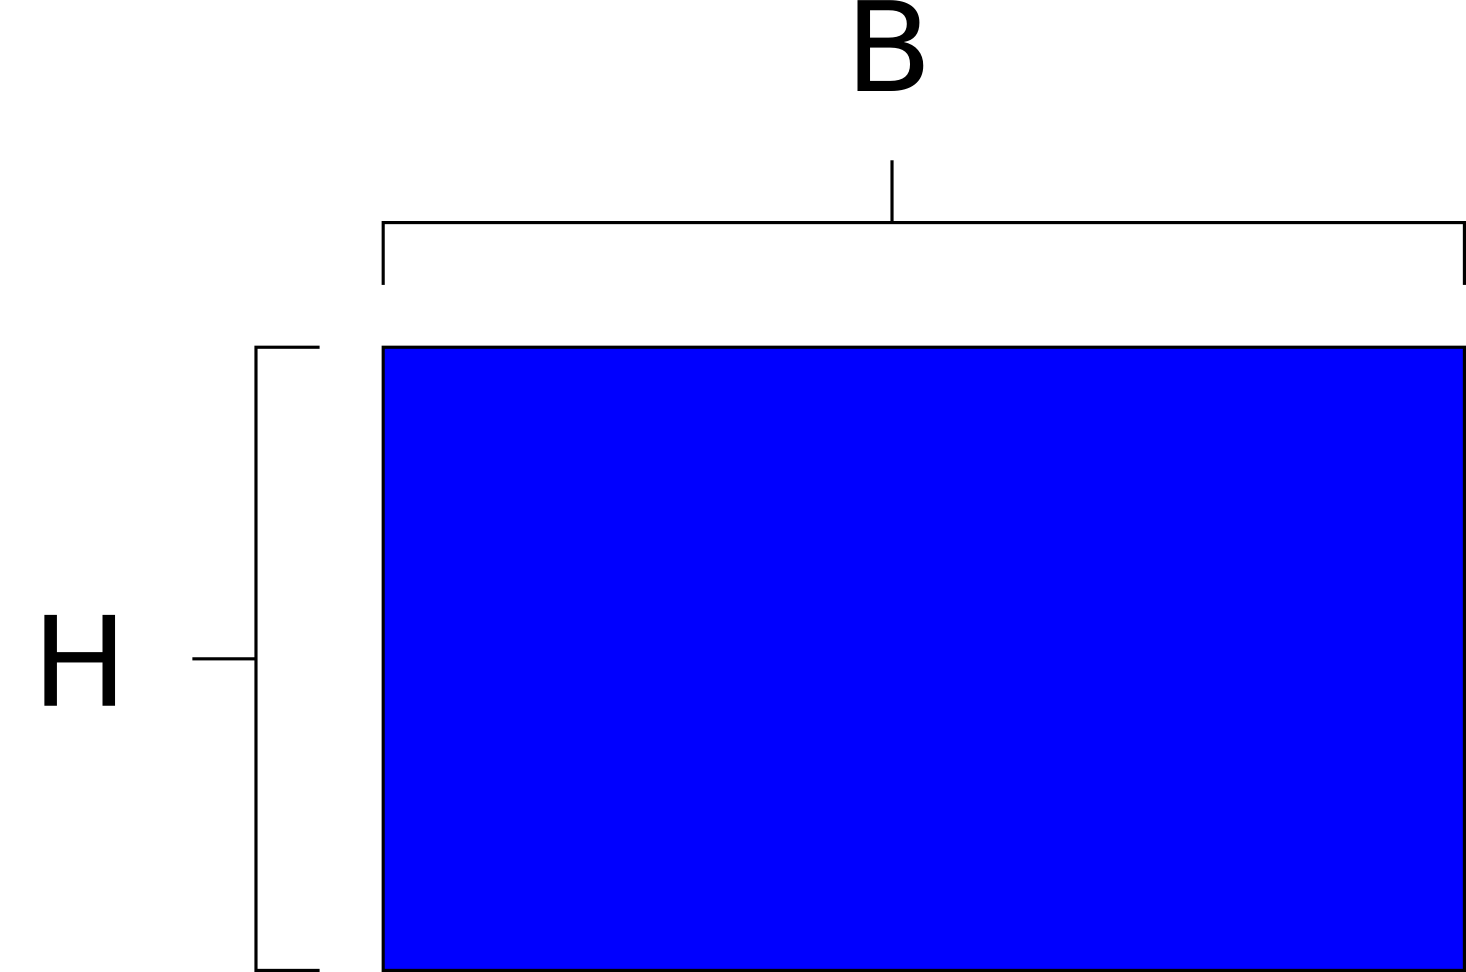
\includegraphics[scale=0.42,angle=0]{afsnit/vores_implementation/billeder/naiv_algoritme/path2407}
	\end{center}
	\caption[]{Billedet opbygning}
	\label{box}
\end{figure}

B og H bliver divideret med $\varPhi$ som giver to tal som betegner, hvor
mange pixels fra begge kanter, det gyldne snit befinder sig f.eks ved et
billedet, som har B = 4000 pixel, vil punktet ligge ved.

\begin{figure}[h]
	\begin{center}
		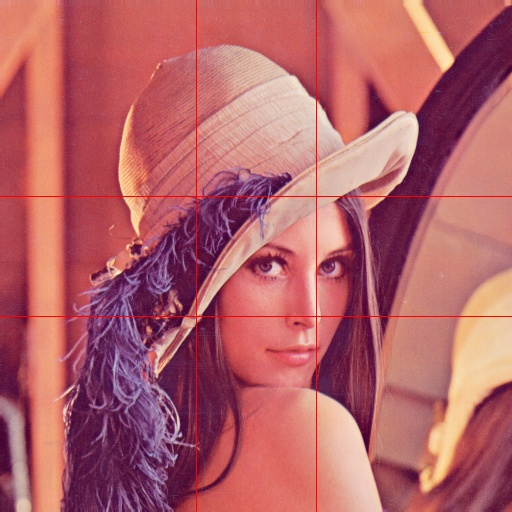
\includegraphics[scale=0.42,angle=0]{afsnit/vores_implementation/billeder/naiv_algoritme/Lenagolden}
	\end{center}
	\caption[]{Billedet som har indtegnet de fire gyldne snit}
	\label{lenasnit2}
\end{figure}

I vores implementering af dette har vi give de 4 forskelige cut vær
deres id 'cut 1 - 4' se figur \ref{cut}, vi vil i reste af raporten
referet til dem ud fra deres id

\begin{figure}[h]
	\begin{center}
		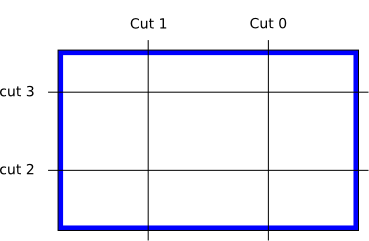
\includegraphics[scale=0.42,angle=0]{afsnit/vores_implementation/billeder/naiv_algoritme/Cut}
	\end{center}
	\caption[]{Billedet hvor de 4 cut er navngivet}
	\label{cut}
\end{figure}

Hvis cutRatio er pracics 0.5 kommer cuttet til at ligge oven i hinanden, og kun skabe 2 cut i steden for firere. id for disse 2 snit er cut 0 og cut 1. ilustret i figur \ref{2Cut}

\begin{figure}[h]
	\begin{center}
		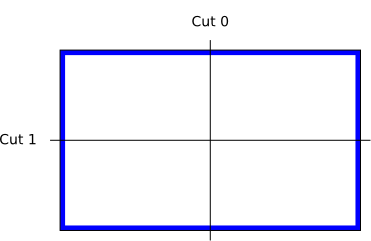
\includegraphics[scale=0.42,angle=0]{afsnit/vores_implementation/billeder/naiv_algoritme/2Cut}
	\end{center}
	\caption[]{cutRation er 0.5, og skaver derfor kun 2 cuts}
	\label{2Cut}
\end{figure}

\subsubsection*{Heltal i det gyldne snit}

\begin{equation}
	4000/\varPhi = 4000(\sqrt{5}-1)/2 = 2472.13595 \approx 2472
\end{equation}

Eksemplet med 4000 pixels ovenfor, approksimationen vi antal pixels ved at
runde resultatet, dette gør at vi mister 0.13595 nøjagtighed, dette svare
til en misvisning af punktet på 0.00339875 $\%$ i forholdt til bredden på
billedet. 

\begin{equation}
	0.13595/4000*100 = 0.00339875
\end{equation}

Det er en maget lille del af selve billedet og skulle ikke give nogle
misvisninger i forhold til udregningen. For at gøre det lidt mere
generat, sætter vi den mistet nøjagtighed til 0.5, det er den maximale
afrundings factor som kan forekommer. Sætter billedet størrelse til 500
pixels, som er det miste billedet vi har, dette giver en fejl margen på
0.1 $\%$, Dette tal bliver adderet til fejl satsen ovenfor og vi kommer
til at at se at det er en ok afrundning af snittet, som ikke kommmer til
at give nogle problemer. 

\subsubsection{Heltal ved udregning af Margin}
En af vores mål ved denne opgave er at se om kunstnern har tegnet
interessante regioner ved opdelingen af billedet ved et gyldne snit og og
samme line det med $\frac{2}{3}$. Da de 2 snit ligger meget tæt på
hinanden og vi gerne vil lave en sammenligning, er det vigtigt at margin
for snittet ikke krydser hinanden. Da dette vil indebære at de samme
region vil blive fundet af begge snit, og vil give et skævt billedet
af forskellen på de to snit.
hvis x betegner antal pixels i B eller H, og vi vil se
forskellen mellem 2/3 og $\varphi$, multiplisere vi x med snittet for at finde
dens placering og subtrahere dem fra hinanden.

\begin{eqnarray}
	\frac{x2}{3}-\frac{x2}{\sqrt{5}+1} &=& x(\frac{2}{3}-\frac{2}{\sqrt{5}+1}) \\ \nonumber
	&=& x(0.666667-0.618034) \\ \nonumber
	&=& x(0.048633) \\
\end{eqnarray}

Vi har nu fundet antal pixels mellem de to snit. Da vi gerne vil undgå at de to
marginens ikke krydser hinanden, dividere vi med 2 og tager en floor på
helle funktionen.

\begin{equation}
	\lfloor(0.048633x/2)\rfloor = 0.024316x
\end{equation}

Dette giver os et antal pixels som skildre de to snit. For at vise
hvor stort marginen egentlige kan være, bruger jeg denne formel på to
billeder, et som svare til vores mindste billedet, 500 pixels, og et
som svare til vores største billedet, 4000 pixels. Ved 500 pixels
bliver resultatet

\begin{equation}
	 \lfloor 500(0.024316)\rfloor = 12
\end{equation}

Dette er en ok margin, da vores fejl på udregningerne ligger på 2.1 \%,
som svare til $500*0.021 = 10.5$ pixels, som er 1.5 pixels fra vores
margin

Ved 4000 pixels giver det.

\begin{equation}
	 \lfloor 4000(0.024316)\rfloor = 97
\end{equation}

som også er god nok da 4000*0.021 = 84 pixels
% vim: set tw=72 spell spelllang=da:
